\documentclass{article}
\usepackage{listings}
\usepackage{graphicx}
\usepackage{hyperref}
\usepackage{xcolor}
\usepackage{amsmath}

\definecolor{codegreen}{rgb}{0,0.6,0}
\definecolor{codegray}{rgb}{0.5,0.5,0.5}
\definecolor{codepurple}{rgb}{0.58,0,0.82}
\definecolor{backcolour}{rgb}{0.95,0.95,0.92}

\lstdefinestyle{mystyle}{
    backgroundcolor=\color{backcolour},   
    commentstyle=\color{codegreen},
    keywordstyle=\color{magenta},
    numberstyle=\tiny\color{codegray},
    stringstyle=\color{codepurple},
    basicstyle=\ttfamily\footnotesize,
    breakatwhitespace=false,         
    breaklines=true,                 
    captionpos=b,                    
    keepspaces=true,                 
    numbers=left,                    
    numbersep=5pt,                  
    showspaces=false,                
    showstringspaces=false,
    showtabs=false,                  
    tabsize=2
}

\lstset{style=mystyle}

\title{ChildSynth: Leveraging Synthetic Imagery for Automated Height Measurement in Malnutrition Prediction}
\author{David Berthiaume}

\begin{document}

\maketitle


\section{Introduction}

Predicting childhood malnutrition is a critical task in the field of public health. Malnutrition among children is still a significant public health problem in many developing countries. It is a primary cause of morbidity and mortality in children. Malnutrition is a condition that results from eating a diet in which one or more nutrients are insufficient, such that the diet causes health problems.

This paper proposes a novel approach to predict malnutrition in children using synthetic imagery. 
We leverage the power of synthetic data to help evaluate and train several deep-learning models to predict heights in children to support the prediction of malnutrition. 

Obtaining data for training deep learning models is a challenging task. The data must be labeled and annotated, which can be time-consuming and expensive. Obtaining images of children to train a model to predict malnutrition is even more challenging. These images and height measurements must be taken in a controlled environment with trained personnel to ensure high accuracy. Furthermore, this data is highly sensitive since it involves images of children.

To combat these challenges, a synthetic data generator, ChildSynth, was developed to create images of children with pixel-perfect height measurements. This synthetic data generator can create an unlimited number of images of children with varying characteristics and pixel-perfect heights. The generated synthetic data can be used to evaluate and pre-train deep learning models to predict children's height. 

\section{ChildSynth}

ChildSynth is a command-line program that uses procedural modeling and, powered by Pov-RAY~\cite{povray}, to generate color images, depth maps, segmentation maps, keypoints, precise height measurements, and auxiliary information for synthetic children lying on a mat as viewed from different camera angles. The following example command generates RGB images, depth maps, segmentation maps, and auxiliary text files with height measurements and other characteristics for $5$ different camera angles for a total of $15$ images. 

\begin{lstlisting}[language=bash]
python render_children.py --resy 512 --resx 512 --num_children 1     --output_dir ./output 
\end{lstlisting}

Figure \ref{fig:child_0} shows an example of a synthetic child generated by the above command.

\begin{figure}[]
    \centering
    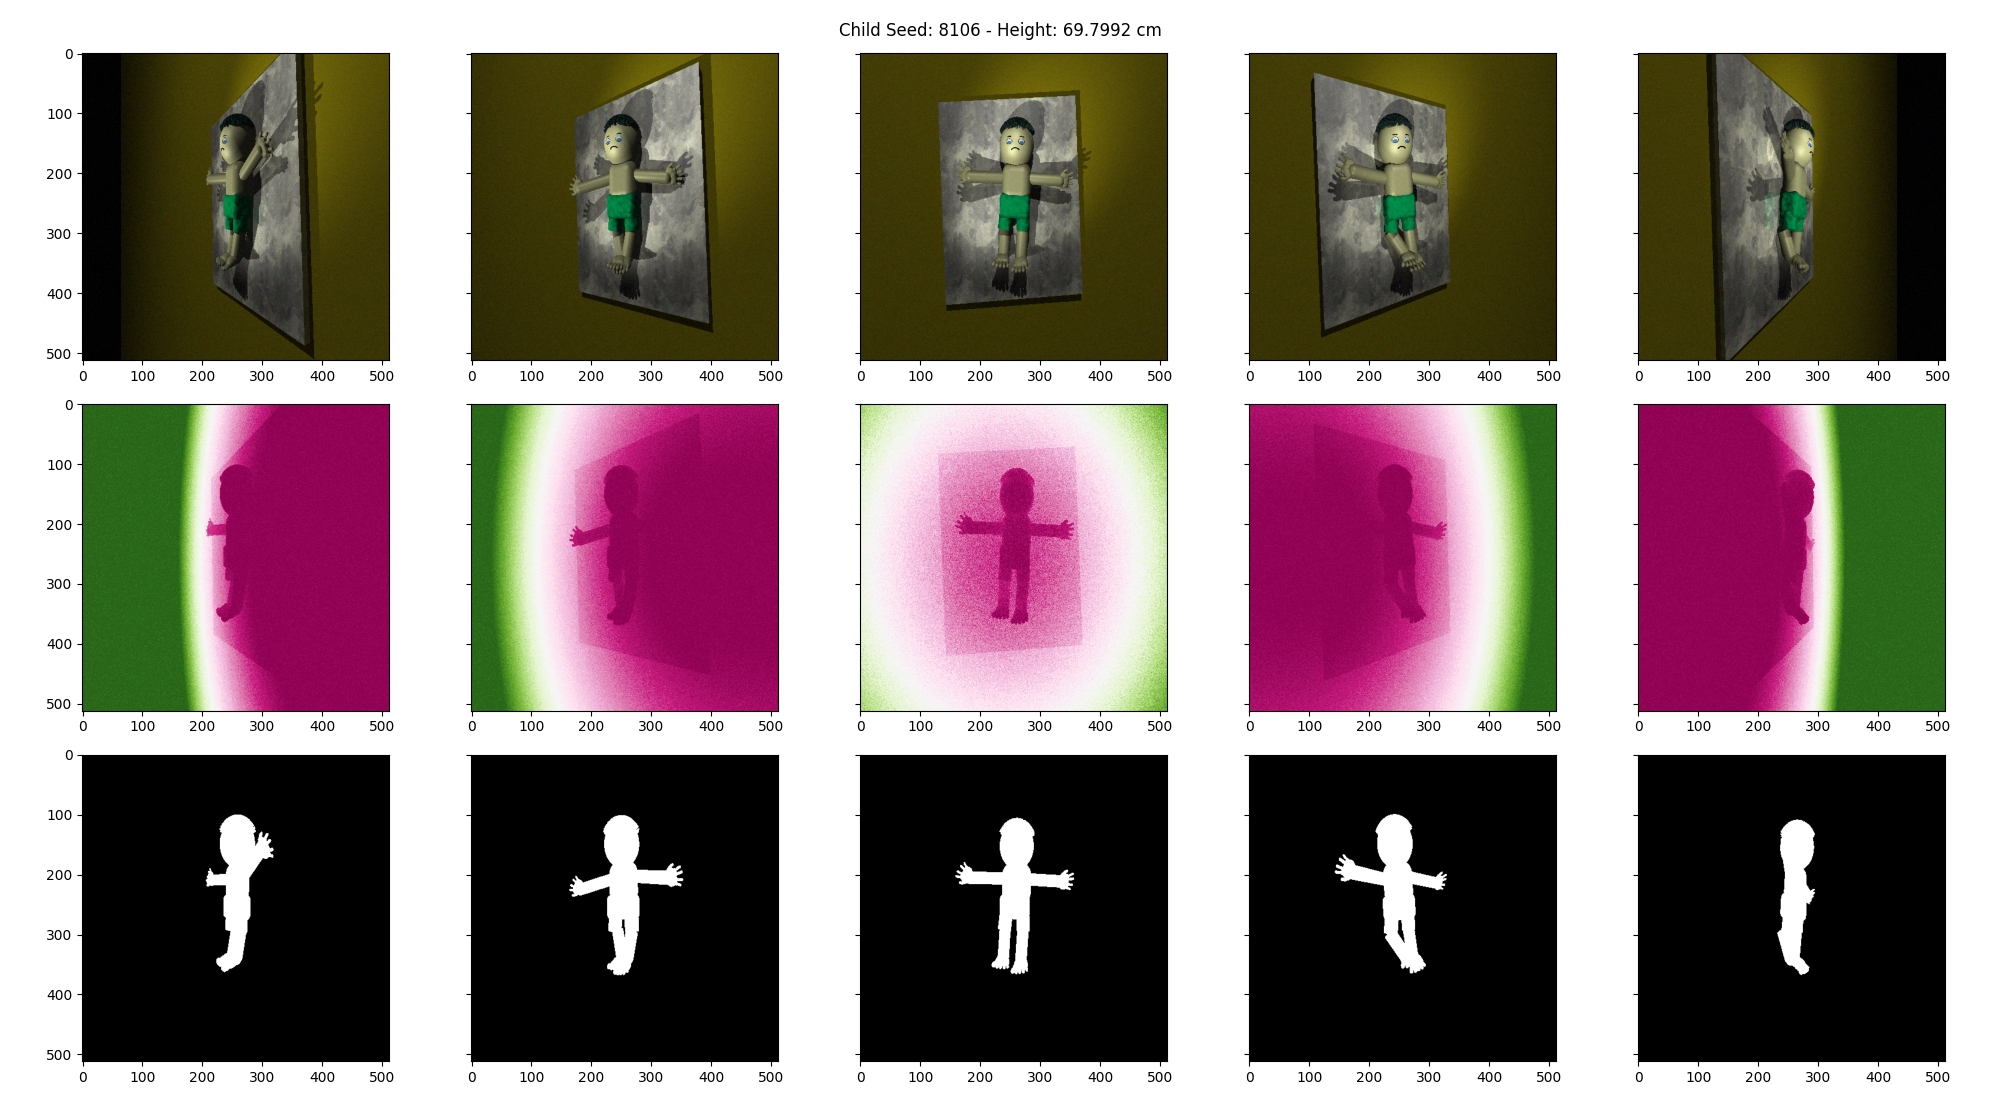
\includegraphics[width=\textwidth]{plots/child_0.png}
    \caption{Example of a synthetic child generated by ChildSynth. The upper row consists of color images, the middle row consists of depth maps, and the bottom row consists of binary segmentation maps indicating whether each pixel is part of a child or part of the background.}
    \label{fig:child_0}
\end{figure}

The goal of ChildSynth is \textbf{not} to generate photorealistic images but to parametrically model children with infinite variations and with pixel-perfect measurements. Every element, the length, style, density, and color of hair, the facial characteristics, the skin and mat textures, even the size of each toe, is modeled parametrically and can be individually specified or sampled from various random distributions. Elements of the scene, including camera position, lighting, and image quality, are also parametrically modeled. One can specify over $100$ different parameters to control how the children and scenes are rendered. Using realistic static meshes, or generative AI would greatly reduce this flexibility and make it difficult to generate the vast number of images with precise and exhaustive measurements needed to train a deep-learning model.

\section{Approach}
\subsection{Rendering}

ChildSynth renders Each parametrically modeled scene using ray tracing. The geometries in the scene are composed of spheres, cylinders, cubes, rounded cubes, planes, and BLOBs (Binary Large OBjects). BLOBs themselves are composed of cubes, cylinders, and spheres and allow one to parametrically create smooth shapes, such as those found in a child's body. A smooth field is created from the multiple component objects within each bloc. Each component of a blob exerts a field in the space around it, and the sum of these fields determines the shape of the blob. When the combined field strength at any point in space exceeds a given threshold value, the surface at that point becomes part of the blob. These composite objects are beneficial for creating smooth shapes parametrically with fine-grained control over the individual features of the shape. Much of the complexity of the child's body is modeled using BLOBs, especially for the feet and hands (see figure \ref{fig:hand_foot}). 

\begin{figure}[htbp]
    \centering
    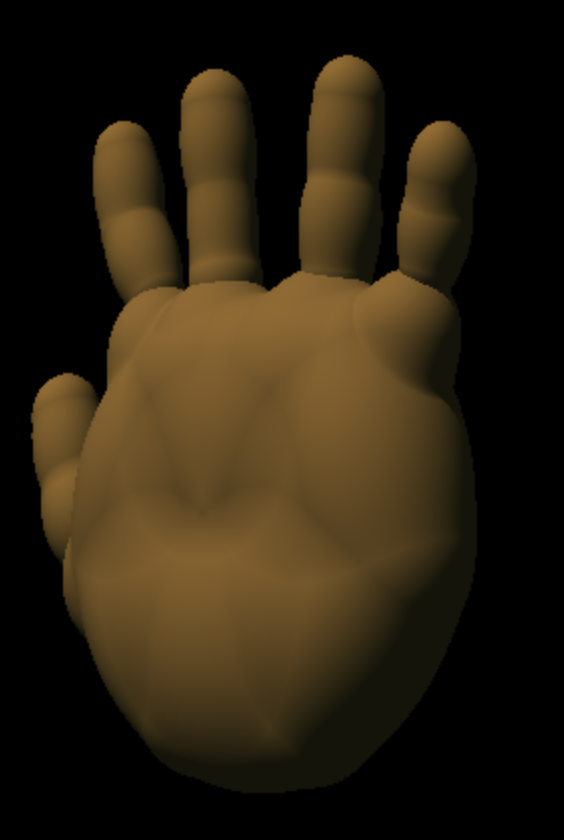
\includegraphics[height=4cm]{plots/hand.png}
    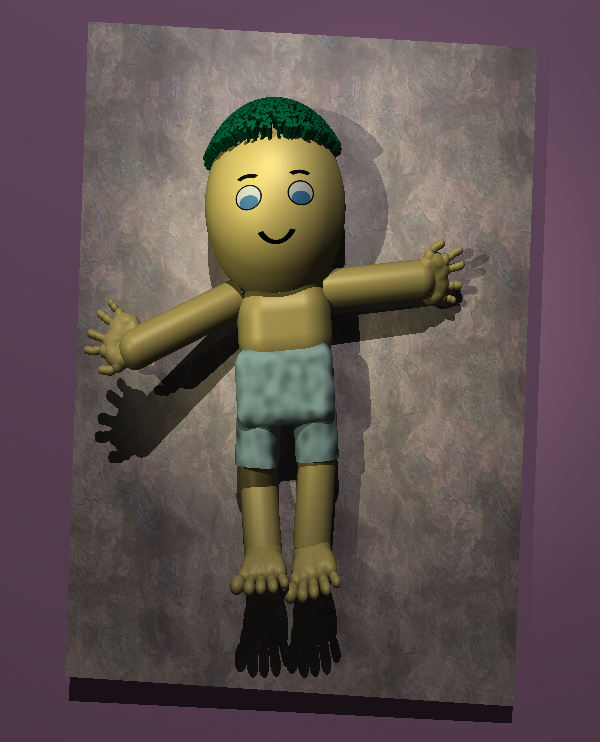
\includegraphics[height=4cm]{plots/back.png}
    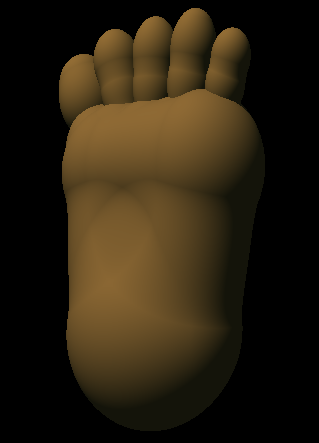
\includegraphics[height=4cm]{plots/foot.png}
    \caption{Hands and feet are rendered using blobs that consist of a complex arrangement of parametric spheres and cylinders. The strength and shape of each sphere and cylinder can be individually controlled to create a wide variety of shapes from the resulting field.}
    \label{fig:hand_foot}
\end{figure}

Each child is rendered from multiple view angles to provide a variety of perspectives. The camera is placed at different positions above the child to capture the child's body from multiple positions. By default, $5$ different camera angles are used to render each child, from $30$ to $150$ degrees, in increments of $30$ degrees, with $90$ degrees being directly above the child, and $30$ and $150$ degrees being to the left and right of the child respectively. These multiple views allow one to predict the child's height with computer vision.

ChildSynth renders a depth image corresponding to each color image by storing the distance from the camera to the scene. The depth image and the color imagery are precisely coregistered.

Finally, ChildSynth renders a segmentation map for each child. The segmentation map is a binary image where each pixel is equal to $0$ if it part of the background and $1$ if it is part of the child. Along with the color and depth images, the segmentation map is helpful for training deep-learning models to predict the child's height.


\subsection{Modeling}

\subsubsection{Randomness}

ChildSynth can render millions of synthetic children, with no two being identical.  It accomplishes this by sampling over $60$ parameters from various probability distributions. For example, ChildSynth may place an optional spotlight around the child as a light source. The position of this spotlight is sampled from several normal distributions, with the light being most likely placed near the child. The color of this light source is sampled from three uniform distributions, one for each of the red, green, and blue intensities. 

Several distributions are available in ChildSynth; all parameters can be optionally specified in the command line and support every probability distribution. Every parameter has a default distribution that is used when no distribution is explicitly provided.

\subsubsection{Probability Distributions}

This section provides a summary of the available probability distributions and their arguments. The following distributions are available in ChildSynth:

\begin{itemize}

    \item {\textbf{Constant}: The simplest distribution defines a single constant value that is selected with probability $1$.}
    
    Example usage:
    \begin{lstlisting}[language=bash]
        python render_children.py --smile_factor constant:0.7 \end{lstlisting}
    
    \item \textbf{Bernoulli}: The Bernoulli distribution defines a probability $p$ that a binary random variable is equal to $1$. This can be used to turn on or off features such as an individual light source, or the rendering of hari. Example usage: \textbf{bern:0.5} 
    
    Example usage:
    \begin{lstlisting}[language=bash]
        python render_children.py --spotlight_1 bern:0.3\end{lstlisting}
   
    \item \textbf{Uniform}: The uniform distribution is defined by two parameters, $a$ and $b$, which are the minimum and maximum values of the distribution. 
    
    Example usage:
    \begin{lstlisting}[language=bash]
        python render_children.py --hair_color_red unif:0.1,0.6\end{lstlisting}
    
    \item \textbf{Normal}: The normal distribution is defined by two parameters, $\mu$ and $\sigma$, which are the mean and standard deviation of the distribution.
    
    Example usage:
    \begin{lstlisting}[language=bash]
        python render_children.py --head_size normal:0.8,0.2\end{lstlisting}
    
    \item \textbf{Binomial}: The binomial distribution is used to sample an integer obtained from $n$ independent Bernoulli samples with probability $p$. This returns the number of successes in these independent trials. To use this distribution, one specifies the number of trials $n$, and then the probability of success for each independent trial $p$. 
    
    Example usage:
        \begin{lstlisting}[language=bash]
        python rener_children.py  --clothes_wrinkles binom:100,0.5\end{lstlisting}

        
\end{itemize}

\subsection{Colors}
ChildSynth supports the specification of colors using the RGB color space where each of the red, green, and blue values lie in the range $[0,1]$. Each channel is specified separately using subparameters separated by an underscore to allow maximum flexibility. The following example specifies the color of hair with a red intensity of $1$, a blue intensity of $0.25$, and a green intensity sampled from a normal distribution with a mean of $0.2$ and a standard deviation of $0.1$. See figure \ref{fig:red_hair}.


\begin{lstlisting}[language=bash]
python render_children.py --hair_color_red 1 --hair_color_blue 0.25 --hair_color_green normal:0.5,0.1\end{lstlisting}

\begin{figure}[htbp]
    \centering
    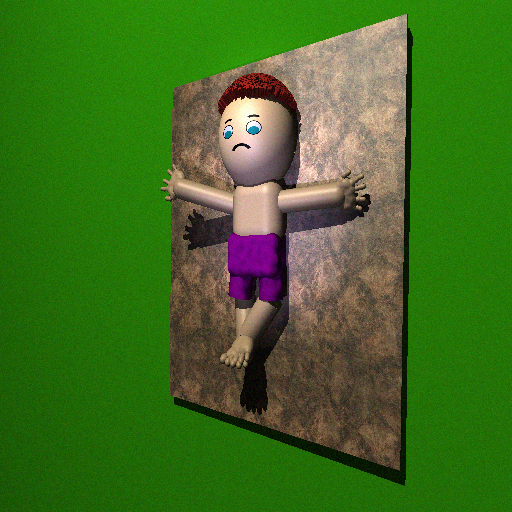
\includegraphics[height=3.7cm]{plots/child_000000_rgb_060.png}
    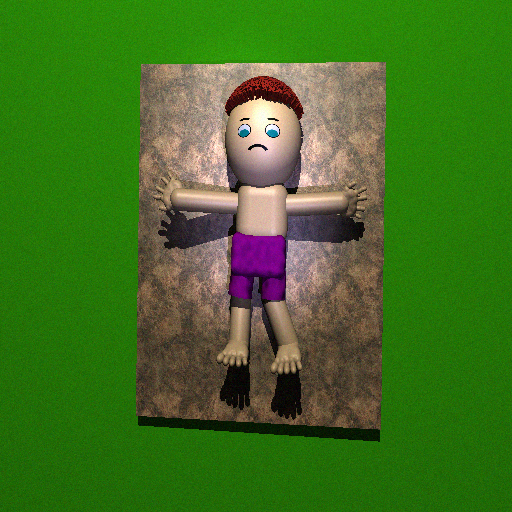
\includegraphics[height=3.7cm]{plots/child_000000_rgb_090.png}
    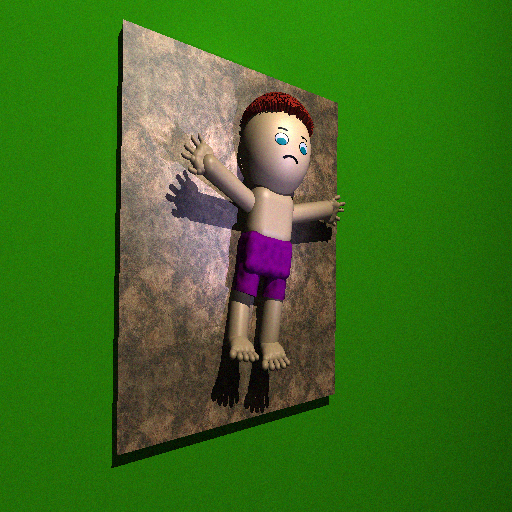
\includegraphics[height=3.7cm]{plots/child_000000_rgb_120.png}
    \caption{Hair color is specified with red, green, and blue intensities. The red and blue intensities are set to $1$ and $0.25$, respectively, while the green intensity is sampled from a normal distribution with a mean of $0.2$ and a standard deviation of $0.1$.}
    \label{fig:red_hair}
\end{figure}

\subsection{Vectors}

ChildSynth similarly supports specifying vectors with subcomponents. For example, one can rotate the child along the x,y, and z axes. To rotate the child $180$ degrees along the z-axis (the z-axis points into the scene) and perform a random translation along the x-axis, one can use the following syntax. See figure \ref{fig:rotation}.


\begin{lstlisting}[language=bash]
python rener_children.py  --child_rotate_z constant:3.1415 --child_shift_x unif:-1.0,1.0\end{lstlisting}

\begin{figure}[htbp]
    \centering
    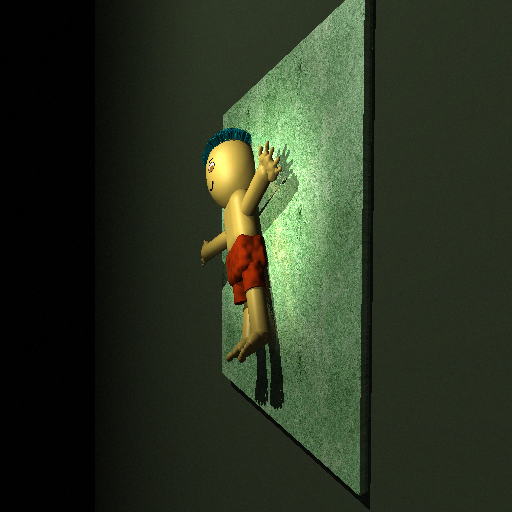
\includegraphics[height=3.7cm]{plots/child_000000_rgb_030a.png}
    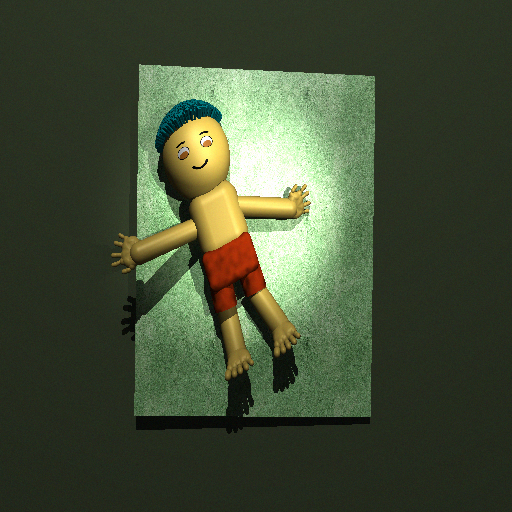
\includegraphics[height=3.7cm]{plots/child_000000_rgb_090a.png}
    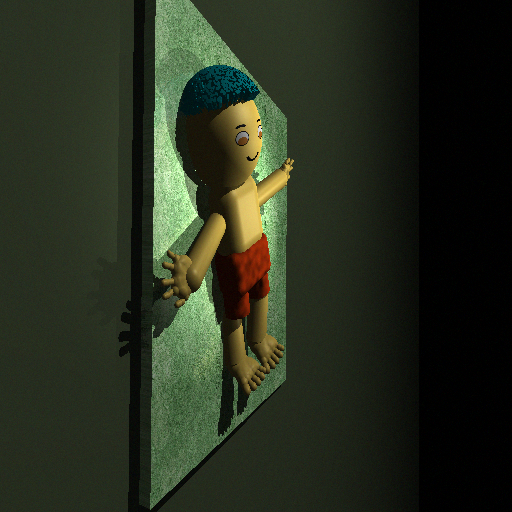
\includegraphics[height=3.7cm]{plots/child_000000_rgb_150a.png}
    \caption{Rotating the child and providing a random shift in the x-direction}
    \label{fig:rotation}
\end{figure}

By combining shifting with rotation, we obtain an image of a child standing on the mat.

\begin{figure}[htbp]
    \centering
    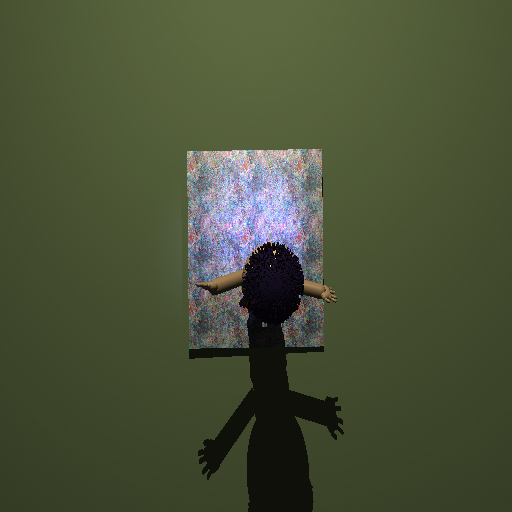
\includegraphics[height=3.7cm]{plots/child_000000_rgb_090c.png}
    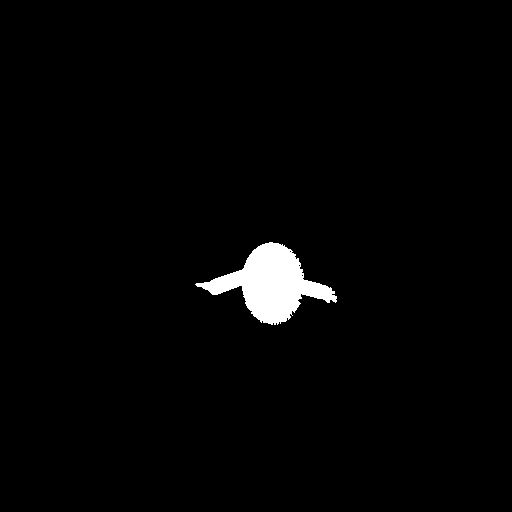
\includegraphics[height=3.7cm]{plots/child_000000_seg_090c.png}
    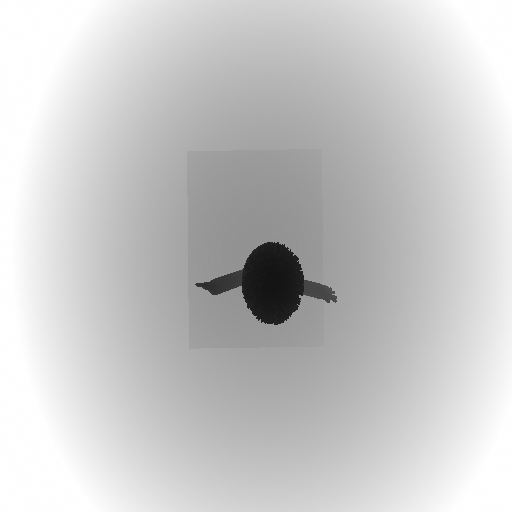
\includegraphics[height=3.7cm]{plots/child_000000_dpt_090c.png}
    \caption{Using a combination of shift and rotation allows us to obtain an image of a child standing on the mat instead of lying down.}
    \label{fig:standing}
\end{figure}

\begin{lstlisting}[language=bash]
render_children.py --child_rotate_x constant:-90 --child_shift_z constant:0.9 --child_shift_y constant:0.4 --camera_distance constant:11\end{lstlisting}

\section{Geometry}

\subsection{BLOBs (Binary Large OBjects)}

Most of the geometry of the synthetic children is composed of BLOBs. BLOBs are a powerful tool for creating smooth shapes parametrically with ray tracing.

BLOBs are created from one or more subcomponents, each typically defined by a field of influence. These fields influence the density of the medium at their respective locations. When combined, they create a smooth surface based on a density threshold, meaning the surface of the blob is defined wherever the combined density of all influence spheres exceeds this threshold.

For example, consider a simple BLOB composed of two spheres
\begin{itemize}
    \item Sphere 1: Center $c_1 = (0, 0, 0)$, radius $r_1 = 1$, strength $s_1 = 1.5$
    \item Sphere 2: Center $c_2 = (1, 0, 0)$, radius $r_2 = 1$, strength $s_2 = 1.5,$
\end{itemize}
and threshold $t_r$.

The influence functions for each sphere are given by:
$$
f_1(p) = 1.5 \left( 1 - \frac{\| p - (0, 0, 0) \|^2}{1^2} \right)^2 \quad \text{if} \quad \| p - (0, 0, 0) \| \leq 1
$$
$$
f_2(p) = 1.5 \left( 1 - \frac{\| p - (1, 0, 0) \|^2}{1^2} \right)^2 \quad \text{if} \quad \| p - (1, 0, 0) \| \leq 1
$$

The total strength at any point $p$ is:
$$
S(p) = f_1(p) + f_2(p)
$$
The points, $p$, inside the BLOB are all $p$ such that $S(p) \geq t_r$.

Blobs can consist of spheres and cylinders, and the strength and shape of each sphere and cylinder can be individually controlled to create a wide variety of shapes from the resulting field.

\begin{figure}[]
    \centering
    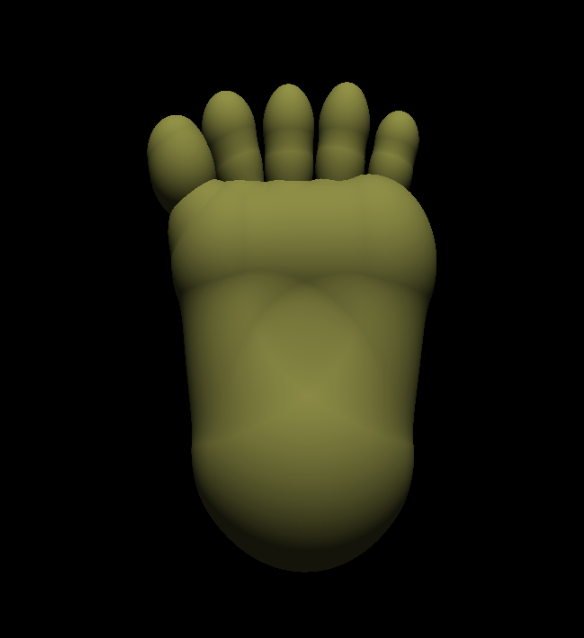
\includegraphics[width=.4\textwidth]{plots/foot2.png}
    \caption{A child's foot is composed of a BLOB that consists of a complex arrangement of parametric spheres and cylinders. The location, size, strength, and shape of each sphere and cylinder are randomly sampled from carefully selected random distributions to create variations in the organic shape of a child's foot while maintaining the general shape that is expected of a standard foot.}
    \label{fig:child_0}
\end{figure}

\subsection{Hierarchical Modeling}
ChildSynth uses a hierarchical modeling approach to create the child's body, with a central skeleton and parametric definitions for parent-child relationships. 

\section{Reference}

Table \ref{table:defaults} lists all the available parameters and their default sample distributions.

\begin{table}[h]
    \centering
    {\scriptsize
    \begin{tabular}{|l|l|l|l|}
    \hline
    \textbf{Parameter} & \textbf{Distribution} & \textbf{Parameters} & \textbf{Description} \\ 
    \hline
    \texttt{head\_size} & normal & 0.8, 0.2 & The size of the head\\ 
    \texttt{skin\_color} & color & (1, 0.8, 0.6), (0.1, 0.1, 0.1) & RGB skin color\\ 
    \texttt{shorts\_color} & color & (0.5, 0.5, 0.5), (0.5, 0.5, 0.5) & RGB shorts color \\ 
    \texttt{mat\_texture} & integer & 101, 200 & Mat texture name \\ 
    \texttt{camera\_distance} & normal & 6.2, 0.2 & Distance of camera to child \\ 
    \texttt{rotation\_adj} & normal & 0.0, 4.0 &  Arm rotation adjustment\\ 
    \texttt{right\_arm\_angle\_xy} & normal & 0.0, 10.0 &  Right arm rotation xy\\ 
    \texttt{left\_arm\_angle\_xy} & normal & 0.0, 10.0 &  Left arm rotation xy\\ 
    \texttt{right\_arm\_angle\_z} & normal & 0.0, 5.0 &  Right arm rotation z\\ 
    \texttt{left\_arm\_angle\_z} & normal & 0.0, 5.0 &  Left arm rotation z\\ 
    \texttt{left\_leg\_angle\_xy} & normal & 0.0, 10.0 & Left leg rotation xy  \\ 
    \texttt{right\_leg\_angle\_xy} & normal & 0.0, 10.0 & Right leg rotation xy  \\ 
    \texttt{right\_leg\_angle\_z} & normal & 0.0, 5.0 &  Left leg angle z\\
    \texttt{left\_leg\_angle\_z} & normal & 0.0, 5.0 &  Left leg angle z\\ 
    \texttt{body\_height} & normal & 2.48, 0.16 & Height of main body \\ 
    \texttt{body\_width} & normal & 0.8, 0.1 & Width of the main body \\
    \texttt{body\_depth} & normal & 0.3, 0.1 & Depth of the main body \\
    \texttt{light\_x} & unif & -5.0, 5.0 & X position of primary light  \\ 
    \texttt{light\_y} & unif & -5.0, 5.0 & Y position of primary light \\ 
    \texttt{light\_z} & unif & -5.0, 5.0 & Y position of primary light \\ 
    \texttt{light1} & unif & 0.3, 1.0 & Intensity of light 1 (primary) \\ 
    \texttt{light2} & unif & 0.3, 1.0 & Intensity of light 2 (point light) \\ 
    \texttt{light3} & unif & 0.2, 1.0 & Intensity of light 3 (spotlight 1) \\
    \texttt{light4} & unif & 0.3, 1.0 & Intensity of light 4 (spotlight 2) \\ 
    \texttt{backcolor\_red} & unif & 0.0, 1.0 & Background color red \\ 
    \texttt{backcolor\_green} & unif & 0.0, 1.0 &  Background color green\\ 
    \texttt{backcolor\_blue} & unif & 0.0, 1.0 & Background color blue \\ 
    \texttt{haircolor\_red} & unif & 0.0, 1.0 &  Hair color red\\ 
    \texttt{haircolor\_green} & unif & 0.0, 1.0 & Hair color green \\ 
    \texttt{haircolor\_blue} & unif & 0.0, 1.0 & Hair color blue \\ 
    \texttt{eye\_color\_index} & integer & 0, 9 & Eye color number \\ 
    \texttt{smile\_factor} & unif & -40.0, 100.0 & Smiling factor (100=full smile) \\ 
    \texttt{mat\_rotate\_y} & unif & -2.0, 2.0 & Mat rotation y axis \\ 
    \texttt{mat\_rotate\_z} & unif & -3.0, 3.0 & Mat rotation x axis \\ 
    \texttt{child\_rotate\_y} & normal & 0.0, 6.0 & Child rotation y axis \\ 
    \texttt{child\_rotate\_z} & normal & 0.0, 6.0 & Child rotation z axis \\ 
    \texttt{child\_rotate\_x} & normal & 0.0, 0.01 & Child rotation x axis \\ 
    \texttt{hair\_count} & unif & 250, 4000 & Number of hair follicles \\
    \texttt{hair\_length} & unif & 0.10, 0.18 & Average hair length \\ 
    \texttt{image\_noise\_level} & unif & 0.0, 8.0 & Gaussian image noise level\\ 
    \texttt{image\_box\_level} & unif & 0.0, 0.01 & Box image noise level \\
    \texttt{child\_shift\_x} & unif & -0.05, 0.05 & Child translation x\\
    \texttt{child\_shift\_y} & unif & -0.05, 0.05 & Child translation y\\
    \texttt{child\_shift\_z} & unif & -0.05, 0.05 & Child translation z\\
    \texttt{foot\_size} & unif & 0.15, 0.23 & Foot size\\
    \texttt{hand\_size} & unif & 0.12, 0.21 & Hand size\\
    \texttt{average\_finger\_length} & unif & 0.05, 0.08 & Average finger length\\
    \texttt{average\_toe\_length} & unif & 0.03, 0.05 & Average toe length\\
    \texttt{light\_1\_color\_red} & unif & 0.5, 1.0 & Light 1 color red\\
    \texttt{light\_1\_color\_green} & unif & 0.5, 1.0 & Light 1 color green\\
    \texttt{light\_1\_color\_blue} & unif & 0.5, 1.0 & Light 1 color blue\\
    \texttt{light\_2\_color\_red} & unif & 0.5, 1.0 & Light 2 color red\\
    \texttt{light\_2\_color\_green} & unif & 0.5, 1.0 & Light 2 color green\\
    \texttt{light\_2\_color\_blue} & unif & 0.5, 1.0 & Light 2 color blue\\
    \texttt{light\_3\_color\_red} & unif & 0.5, 1.0 & Light 3 color red\\
    \texttt{light\_3\_color\_green} & unif & 0.5, 1.0 & Light 3 color green\\
    \texttt{light\_3\_color\_blue} & unif & 0.5, 1.0 & Light 3 color blue\\
    \texttt{light\_4\_color\_red} & unif & 0.1, 0.3 & Light 4 color red\\
    \texttt{light\_4\_color\_green} & unif & 0.1, 0.3 & Light 4 color green\\
    \texttt{light\_4\_color\_blue} & unif & 0.1, 0.3 & Light 4 color blue\\
    \texttt{light\_1position\_x} & unif & -5.0, 5.0 & Light 1 position x\\
    \texttt{light\_1position\_y} & unif & -5.0, 5.0 & Light 1 position y\\
    \texttt{light\_1position\_z} & unif & -5.0, 5.0 & Light 1 position z\\
    \texttt{light\_2position\_x} & unif & -5.0, 5.0 & Light 2 position x\\
    \texttt{light\_2position\_y} & unif & -5.0, 5.0 & Light 2 position y\\
    \texttt{light\_2position\_z} & unif & -5.0, 5.0 & Light 2 position z\\

    \hline
    \end{tabular}
    }
    \caption{ChildSynth default parameters}
    \label{table:defaults}
\end{table}



\bibliographystyle{unsrt}
\bibliography{references}


\end{document}